\begin{figure}
  \setlength{\unitlength}{\textwidth}

        \begin{picture}(1,0.5)(0,0.4)

      % % % Parkinson Data 
%      \put(0.1,1.1){\includegraphics[width=0.75\unitlength]{../FnP/gnuplot/displacement_high_pi_1.eps}}
      \put(0.1,0.76){\includegraphics[width=0.75\unitlength]{../FnP/gnuplot/mean_power_high_pi_1.eps}}
      \put(0.1,0.42){\includegraphics[width=0.75\unitlength]{../FnP/gnuplot/mean_power_low_pi_plot2.eps}}
      
         \put(0.05,0.95){$\displaystyle\frac{P_{m}}{\rho \mathcal{A}U^3 }$}
%         \put(0.07,1.3){$\displaystyle\frac{A}{D}$}
         \put(0.05,0.64){$\displaystyle\frac{P_{m}}{\rho \mathcal{A}U^3 }$}
         \put(0.5,0.4){$\massdamp$}



%      
%      \put(0.189,1.415){\small(a)}
      \put(0.189,1.07){\small(a)}
      \put(0.189,0.73){\small(b)}
%  

      
    \end{picture}

 \caption{Dimensionless mean power as a function of \massdamp\ obtained using the QSS model at $\reynoldsnumber=200$. (a) High \massstiff; data presented at four different combined mass-stiffness levels.\ $\massstiff=10 \ (\mstar=20,\ \ustar=40)$ \ ($\times$),\ $\massstiff=100 \ (\mstar=80,\ \ustar=50) \ (+)$,\ $\massstiff=500 \ (\mstar=220,\ \ustar=60)$ \ (\ding{117}) and \ $\massstiff=1000 \ (\mstar=400,\ \ustar=40) \ (\triangle)$. (b) Low \massstiff; data presented at $\massstiff=10 \ (\times)$, \  $\massstiff=0.1 \ $ (\ding{117}), and  \  $\massstiff=0.01 \ \ (\triangle)$.}
    \label{fig:high_pi_1}
\end{figure}

 %vspace{10cm}
